\documentclass[12pt,a4paper]{article}

\usepackage[a4paper,margin=0.72in]{geometry}
\usepackage[T1]{fontenc}
\usepackage[utf8]{inputenc}
\usepackage{newtxtext,newtxmath}
\usepackage{microtype}
\usepackage{enumitem}
\usepackage{booktabs}
\usepackage{tabularx}
\usepackage{ragged2e}
\usepackage{array}
\usepackage{multirow}
\usepackage{graphicx}
\usepackage{tikz}
\usetikzlibrary{arrows.meta,positioning}
\usepackage{titlesec}
\usepackage{needspace}
\usepackage{fancyhdr}
\usepackage[hidelinks]{hyperref}

\setlength{\parindent}{0pt}
\setlength{\parskip}{4pt}
\setlist[itemize]{leftmargin=*,topsep=2pt,itemsep=1pt,parsep=0pt}
\setlist[enumerate]{leftmargin=*,topsep=2pt,itemsep=1pt,parsep=0pt}
\renewcommand{\arraystretch}{1.08}
\setcounter{secnumdepth}{0}
\titleformat{\section}{\fontsize{20}{24}\selectfont\bfseries}{}{0pt}{}
\titlespacing*{\section}{0pt}{13pt}{5pt}
\titleformat{\subsection}{\fontsize{14}{17}\selectfont\bfseries}{}{0pt}{}
\titlespacing*{\subsection}{0pt}{10pt}{4pt}
\pagestyle{fancy}
\fancyhf{}
\fancyfoot[C]{\small\thepage}
\renewcommand{\headrulewidth}{0pt}

\tikzset{
  flow/.style={draw,rounded corners=2pt,align=center,minimum width=0.88\linewidth,
    minimum height=0.56cm,inner sep=4pt,font=\footnotesize},
  arrow/.style={-{Latex[length=1.5mm]},semithick}
}

% Every chapter starts on a new page
\newcommand{\chapter}[1]{%
  \clearpage
  \section*{#1}}

% 18pt bold heading used for ABSTRACT and BIBLIOGRAPHY
\newcommand{\bighead}[1]{%
  {\fontsize{18}{22}\selectfont\bfseries #1}\par\vspace{6pt}}

\begin{document}

%=====================================================================
% TITLE PAGE
%=====================================================================
\thispagestyle{empty}

% Page border
\begin{tikzpicture}[remember picture, overlay]
  \draw[line width=1pt]
    ([xshift=1.2cm,yshift=-1.2cm]current page.north west)
    rectangle
    ([xshift=-1.2cm,yshift=1.2cm]current page.south east);
\end{tikzpicture}

\begin{center}

  \vspace*{0.5cm}

  % Project title
  {\fontsize{20}{24}\selectfont\bfseries PROJECT SYNOPSIS}\\[10pt]

  {\fontsize{21}{25}\selectfont\bfseries
  Evidence-Aware Multimodal Data Integration\\[2pt]
  for Reliable Enterprise Data Consolidation}\\[8pt]

  {\normalsize\itshape Proposed System: DataMesh AI}

  \vspace{1.2cm}

  % Submitted by
  {\fontsize{14}{17}\selectfont A Synopsis Submitted By}\\[10pt]

  {\fontsize{14}{17}\selectfont\bfseries
  Archit Jain (2415800016)}\\[3pt]

  {\fontsize{14}{17}\selectfont\bfseries
  Deepti Yadav (2415800029)}

  \vspace{1.0cm}

  % Degree
  {\fontsize{12}{15}\selectfont\itshape
  The Semester Project Report submitted in partial fulfilment of the}\\[3pt]

  {\fontsize{12}{15}\selectfont\itshape
  requirements for the award of the degree of}

  \vspace{0.45cm}

  {\fontsize{18}{21}\selectfont\bfseries
  Bachelor of Technology}\\[2pt]

  {\fontsize{18}{21}\selectfont\bfseries
  (Honors)}

  \vspace{0.25cm}

  {\fontsize{14}{17}\selectfont in}\\[4pt]

  {\fontsize{15}{18}\selectfont\bfseries
  Computer Science and Engineering}

  \vspace{1.2cm}

  
\includegraphics[width=2.2in]{image1.png}\\[10pt]
  % Department and university
  {\fontsize{14}{17}\selectfont
  Department of Computer Engineering and Applications}\\[4pt]

  {\fontsize{15}{18}\selectfont\bfseries
  GLA University, Mathura, UP}\\[4pt]

  {\fontsize{14}{17}\selectfont
  August, 2026}

\end{center}

\newpage

%=====================================================================
% CHAPTER 1: INTRODUCTION
%=====================================================================
\chapter{CHAPTER 1: INTRODUCTION}\label{page:ch1}

\subsection*{1.1 What is Multimodal Data Integration?}

Modern enterprise environments store business-critical information across fragmented and heterogeneous modalities, including relational tables, Excel spreadsheets, CSV exports, PDF reports, scanned receipts, and semi-structured documents. A single customer, transaction, or product entity frequently appears across disparate files with differing attribute names, conflicting numerical values, heterogeneous currency representations, and asynchronous reporting dates. While modern vision-language models (VLMs) and Optical Character Recognition (OCR) systems can perform localized structured extraction from documents, extraction alone does not resolve the data integration challenge.

A reliable consolidation system must establish whether distinct extracted fields share common semantic attributes (schema matching), determine whether separate records refer to the exact same real-world entity (entity resolution), systematically resolve conflicting values (data fusion), and provide transparent provenance tracking for every fused attribute.

Recent literature published in premier journals has examined these subproblems: multi-signal feature fusion for schema matching \cite{smutf2025}, error propagation and cluster repair in entity resolution \cite{christen2025cluster}, false-discovery estimation in record linkage \cite{robach2025falsediscovery}, multi-stage table integration and conflict resolution \cite{ji2025tableintegration}, classifier calibration \cite{silvafilho2023calibration}, multi-granular data provenance \cite{gregori2025prolit}, and tabular foundation models for downstream prediction \cite{hollmann2025tabpfn}. However, existing systems lack an integrated, evidence-aware decision layer that propagates structural signals, source provenance, temporal freshness, and cross-source consensus to prevent catastrophic false merges.

\subsection*{1.2 Proposed System Modules}

The proposed system, \textbf{DataMesh AI}, addresses this limitation through four core architectural modules:

\begin{itemize}
  \item \textbf{Multimodal Ingestion and Extraction.} Ingests heterogeneous business artifacts (PDFs, scanned invoices, XLSX, CSV). Multimodal foundation models (e.g., Qwen) and specialized document parsers extract tabular and key-value records while recording bounding-box locations, extraction confidence scores, and format metadata.
  \item \textbf{Evidence Representation and Construction.} For every candidate schema correspondence, entity pair, and value candidate, the system extracts a composite seven-dimensional evidence vector spanning semantic similarity, structural compatibility, value-pattern match, entity co-reference, source provenance, temporal freshness, and cross-source agreement.
  \item \textbf{Evidence-Aware Reconciliation and Decision Layer.} Rather than forcing an uncalibrated binary merge, a lightweight calibrated decision model computes probabilistic confidence over candidate mappings, outputting one of four risk-sensitive actions: \textbf{MERGE}, \textbf{REVIEW}, \textbf{REJECT}, or \textbf{ABSTAIN}.
  \item \textbf{Selective Output and Downstream Verification.} Emits an auditable canonical structured dataset complete with cell-level provenance trails and routes ambiguous records to a human review queue. The resulting consolidated dataset is verified for utility on downstream tabular machine learning tasks.
\end{itemize}

\subsection*{1.3 System Architecture}

Figure~1 depicts the systematic pipeline of DataMesh AI, tracking information flow from raw heterogeneous inputs through multimodal extraction, multi-signal evidence aggregation, calibrated decision policies, and canonical dataset delivery.

\begin{center}
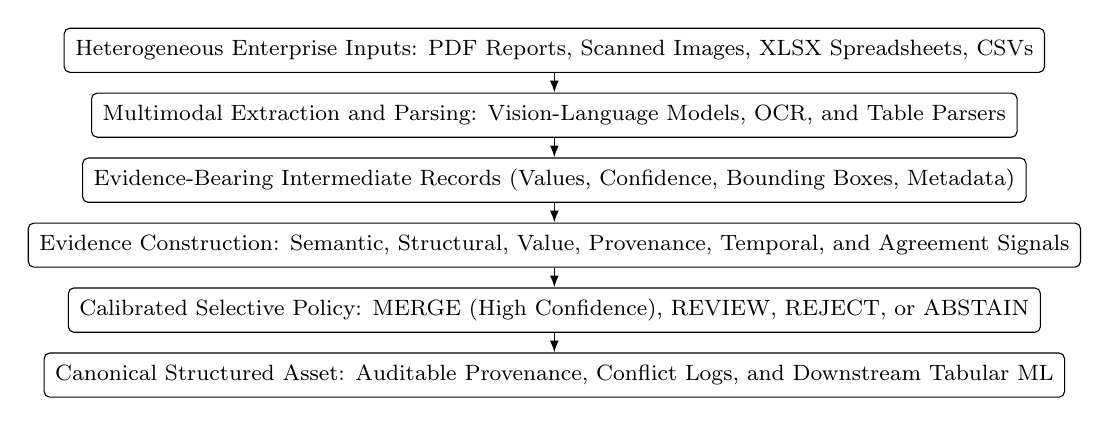
\begin{tikzpicture}[node distance=2.5mm]
  \node[flow] (input) {Heterogeneous Enterprise Inputs: PDF Reports, Scanned Images, XLSX Spreadsheets, CSVs};
  \node[flow,below=of input] (extract) {Multimodal Extraction and Parsing: Vision-Language Models, OCR, and Table Parsers};
  \node[flow,below=of extract] (intermediate) {Evidence-Bearing Intermediate Records (Values, Confidence, Bounding Boxes, Metadata)};
  \node[flow,below=of intermediate] (reconcile) {Evidence Construction: Semantic, Structural, Value, Provenance, Temporal, and Agreement Signals};
  \node[flow,below=of reconcile] (decision) {Calibrated Selective Policy: MERGE (High Confidence), REVIEW, REJECT, or ABSTAIN};
  \node[flow,below=of decision] (output) {Canonical Structured Asset: Auditable Provenance, Conflict Logs, and Downstream Tabular ML};
  \foreach \a/\b in {input/extract,extract/intermediate,intermediate/reconcile,reconcile/decision,decision/output}
    \draw[arrow] (\a) -- (\b);
\end{tikzpicture}

\vspace{2pt}
\small Figure 1: Proposed evidence-aware multimodal consolidation architecture (DataMesh AI)
\end{center}

\subsection*{1.4 Research Problem and Hypotheses}

\textbf{Research Problem.} How can heterogeneous business information extracted from disparate document and tabular sources be reconciled into a unified canonical schema and entity representation while systematically preventing incorrect entity merges and unverified data-fusion decisions?

To investigate this problem, the project formulates three core empirical hypotheses:

\begin{itemize}
  \item \textbf{Hypothesis 1 ($H_1$).} A multi-signal reconciliation layer combining semantic, structural, value-level, provenance, temporal, and cross-source agreement evidence achieves higher entity-matching and data-fusion accuracy under conflicting and heterogeneous enterprise source conditions than semantic-only or LLM-only baselines.
  \item \textbf{Hypothesis 2 ($H_2$).} Introducing a calibrated selective abstention policy (MERGE, REVIEW, REJECT, ABSTAIN) significantly reduces false entity merges and selective risk while maintaining acceptable automated consolidation coverage.
  \item \textbf{Hypothesis 3 ($H_3$).} The reduction of false merges and fusion conflicts achieved through evidence-aware consolidation produces measurable accuracy and reliability gains in downstream tabular machine learning models compared with uncurated or direct LLM merges.
\end{itemize}

\subsection*{1.5 Experimental Methodology and Evaluation Variables}

The experimental evaluation benchmarks DataMesh AI across standardized multi-source integration tasks spanning schema matching, value normalization, entity matching, and data fusion. Candidate extraction inputs from documents and spreadsheets are fed under identical conditions to isolate the contribution of each evidence signal.

\textbf{Experimental Variables:}
\begin{itemize}
  \item \textbf{Independent Variables:} Evidence configurations (Semantic-only; Semantic + Structural; Semantic + Value-patterns; Semantic + Provenance/Temporal; Full Multi-signal Evidence Vector).
  \item \textbf{Dependent Variables:} Schema Matching F1-score; Entity Matching Precision, Recall, and F1; Value Normalization Accuracy; Data Fusion Accuracy; False-Merge Rate; False-Split Rate; Coverage vs.\ Selective Risk; Expected Calibration Error (ECE); Brier Score; and End-to-End Canonical Correctness.
  \item \textbf{Downstream Utility Variables:} Downstream tabular prediction accuracy, F1-score, and regression RMSE evaluated on the resulting canonical datasets.
  \item \textbf{System Variables:} End-to-end processing latency, memory footprint, and token/API cost per integrated document.
\end{itemize}

\subsection*{1.6 Implementation Plan}

The six-month implementation schedule is distributed across distinct technical milestones:

\begin{center}
\small
\begin{tabularx}{\linewidth}{@{}p{1.1cm}p{3.2cm}X@{}}
\toprule
\textbf{Period} & \textbf{Phase} & \textbf{Activities and Key Deliverables} \\
\midrule
M1 & Literature and Formalization & Detailed study of peer-reviewed journal literature in schema matching, entity resolution, data fusion, calibration, and provenance; formalize evidence representations and metrics. \\
M2 & Benchmark and Baselines Setup & Prepare integration testbeds across multi-source domains; implement deterministic string, lexical, and embedding-based baselines; verify ground-truth evaluation harness. \\
M3 & Multimodal Extraction Pipeline & Deploy multimodal vision-language model inference and OCR adapters; generate intermediate representations capturing values, cell locations, and extraction confidence. \\
M4 & Evidence Engine and Decision Layer & Implement seven evidence modules; train lightweight calibrated fusion classifier; integrate MERGE, REVIEW, REJECT, and ABSTAIN thresholding policies. \\
M5 & Empirical Evaluation and Ablations & Execute comparative experiments against baselines; perform signal ablation studies ($E_1$ through $E_7$); plot risk-coverage curves and calibration reliability diagrams. \\
M6 & System Packaging and Reporting & Integrate human review queue, provenance visualization dashboard, and canonical database export; finalize documentation, research report, and reproducibility suite. \\
M7--M12 & Optional Extension & Broader scanned-document evaluation, active learning from human feedback, and downstream tabular foundation model benchmarking. \\
\bottomrule
\end{tabularx}
\end{center}

%=====================================================================
% CHAPTER 2: LITERATURE REVIEW
%=====================================================================
\chapter{CHAPTER 2: LITERATURE REVIEW}\label{page:ch2}

This chapter reviews seven recent (2023--2025) peer-reviewed journal papers that establish the theoretical and algorithmic pillars of the proposed system. Table~1 summarizes these methods, their limitations, and the specific advancements introduced by DataMesh AI.

\subsection*{2.1 Related Work and Studied Literature}

The literature review is organized around the core dimensions of multimodal enterprise data consolidation:

\textbf{1. Multi-Signal Schema Matching.}
In \textit{Information Systems}, Zhang et al.\ \cite{smutf2025} introduce SMUTF, a schema matcher that combines generative tags produced by a large language model with hybrid features: lexical column-name features, data-type compatibility, value-distribution similarity, and pre-trained language-model embedding similarity. The signals are fused by a single gradient-boosted classifier that predicts column correspondence. This is the closest published ancestor of the proposed evidence representation, demonstrating that independently computed signals can be combined by a learned model into one matching decision. Its scope is schema-level column matching; it performs no row-level entity resolution or data fusion, and it provides no calibrated confidence or abstention.

\textbf{2. Entity Resolution Errors and False Merges.}
In the \textit{ACM Journal of Data and Information Quality}, Christen et al.\ \cite{christen2025cluster} address the propagation of linkage errors through transitive closure: a single erroneous pairwise link ($A\!\sim\!B$, $B\!\sim\!C$) may merge distinct entities into one cluster with no internal signal that the cluster is incorrect. They detect and repair such clusters using graph-metric features over the linkage graph together with active learning. Their repair operates after the merge has been committed, and the active-learning oracle is a language model rather than a human expert.

\textbf{3. False-Discovery Estimation in Record Linkage.}
In \textit{Statistics in Medicine}, Robach et al.\ \cite{robach2025falsediscovery} propose a method for estimating the false discovery proportion among accepted record links by augmenting a data file with synthetic, non-linkable ``decoy'' records and measuring how many are falsely linked. The procedure requires no ground-truth labels and applies to any linkage algorithm. Their validation is on biomedical and survey record linkage, so transfer to enterprise data requires re-validation; the estimation principle nonetheless provides a principled definition of a False-Merge Rate.

\textbf{4. Multi-Stage Table Integration and Conflict Resolution.}
In \textit{The VLDB Journal}, Ji et al.\ \cite{ji2025tableintegration} present a three-stage integration pipeline for data lakes: pairwise integrability judgment, integrable set discovery, and multi-tuple conflict resolution. The pipeline assumes that input tables have already been schema-aligned into a common intermediate table, and it always emits an integrated tuple, selecting a single value for each conflicting attribute, with no confidence estimate, abstention, or review step.

\textbf{5. Classifier Calibration.}
In \textit{Machine Learning}, Silva Filho et al.\ \cite{silvafilho2023calibration} survey classifier calibration, defining expected calibration error and the Brier score, reliability diagrams, and post-hoc calibration methods including temperature scaling, Platt scaling, isotonic calibration, and Dirichlet calibration for binary and multiclass problems, and releasing the open-source \textit{PyCalib} library. The survey is scoped to calibration under a matched deployment setting and explicitly excludes abstention and out-of-distribution robustness.

\textbf{6. Data Provenance and Auditability.}
In the \textit{Journal of Big Data}, Gregori et al.\ \cite{gregori2025prolit} present an LLM-guided platform for multi-granular data provenance, distinguishing cell-level, column-level, and pipeline-level provenance and supporting lineage queries over the resulting graph. The system records and explains provenance, but it does not consume provenance as an input to any merge or reconciliation decision.

\textbf{7. Downstream Tabular Prediction.}
In \textit{Nature}, Hollmann et al.\ \cite{hollmann2025tabpfn} present TabPFN v2, a tabular foundation model that performs in-context learning over an unseen table in a single forward pass and reports state-of-the-art accuracy on datasets of up to ten thousand samples and five hundred features. Because the model is validated only within that size regime, a gradient-boosted-tree baseline is required for larger canonical tables.

\subsection*{2.2 Comparison of Existing Methods}

\needspace{0.78\textheight}

\begin{table}[htbp]
\centering
\caption{Comparative analysis of studied 2023--2025 peer-reviewed journal papers and proposed advancements}
\label{tab:existing_methods}

\footnotesize
\renewcommand{\arraystretch}{1.25}
\setlength{\tabcolsep}{4pt}

\begin{tabularx}{\textwidth}{
    @{}
    >{\RaggedRight\arraybackslash}p{0.20\textwidth}
    >{\RaggedRight\arraybackslash}p{0.20\textwidth}
    >{\RaggedRight\arraybackslash}p{0.20\textwidth}
    >{\RaggedRight\arraybackslash}X
    @{}
}
\toprule

\textbf{Studied Journal Paper}
&
\textbf{What It Already Solves}
&
\textbf{Limitation Relevant to This Project}
&
\textbf{What This Project Changes and How It Is Evaluated}
\\

\midrule

Zhang et al.\ (2025) \cite{smutf2025} \newline
\textit{Information Systems}
&
Fuses lexical, value-distribution, embedding and LLM-tag features into one learned schema-matching classifier.
&
Column (schema) matching only; no entity resolution, fusion or abstention.
&
Extends multi-signal fusion to row-level merge decisions; scored by Entity F1 and False-Merge Rate.
\\[4pt]

Christen et al.\ (2025) \cite{christen2025cluster} \newline
\textit{ACM JDIQ}
&
Repairs wrong entity clusters formed by transitive closure, using graph metrics and active learning.
&
Repairs after the merge; oracle is an LLM, not a human.
&
Prevents the merge up front via a calibrated review queue; scored by False-Merge Rate at fixed coverage.
\\[4pt]

Robach et al.\ (2025) \cite{robach2025falsediscovery} \newline
\textit{Statist.\ Med.}
&
Estimates the false-discovery proportion of accepted links via synthetic decoy records; label-free.
&
Biomedical data; assumes random links; estimates, not bounds.
&
Adopted as the operational False-Merge Rate for threshold tuning; re-validated on our data.
\\[4pt]

Ji et al.\ (2025) \cite{ji2025tableintegration} \newline
\textit{The VLDB Journal}
&
Three-stage integration: integrability judgment, set discovery, multi-tuple conflict resolution.
&
Assumes tables already schema-aligned; always merges, with no abstention.
&
Extends to end-to-end multi-format input with an evidence-gated merge-or-abstain at each stage.
\\[4pt]

Silva Filho et al.\ (2023) \cite{silvafilho2023calibration} \newline
\textit{Machine Learning}
&
Defines ECE, Brier score, reliability diagrams and post-hoc calibration (temperature, Platt, isotonic, Dirichlet).
&
Calibration only; excludes abstention and distribution shift.
&
Supplies the decision layer's calibration methodology; scored by ECE, Brier and reliability diagrams.
\\[4pt]

Gregori et al.\ (2025) \cite{gregori2025prolit} \newline
\textit{J.\ Big Data}
&
Multi-granular provenance (cell, column, pipeline) with lineage queries.
&
Records provenance only; never feeds it into a merge decision.
&
Uses provenance as evidence dimension E5 in reconciliation, alongside the audit trail.
\\[4pt]

Hollmann et al.\ (2025) \cite{hollmann2025tabpfn} \newline
\textit{Nature}
&
In-context tabular foundation model; strong accuracy on small-to-medium tables.
&
Validated only to 10{,}000 samples / 500 features.
&
Tests whether consolidation improves downstream prediction; adds a boosted-tree baseline beyond that regime.
\\[4pt]

Commercial Baseline \newline
(e.g., Julius AI, direct LLMs)
&
Conversational analysis and visualization of uploaded files.
&
Queries clean tables; no multi-source reconciliation or conflict resolution.
&
Adds an auditable reconciliation layer producing a canonical, provenance-backed dataset.
\\

\bottomrule
\end{tabularx}

\end{table}

\subsection*{2.3 Research Gaps}

Analysis of the studied literature identifies five unresolved research gaps:

\begin{itemize}
  \item \textbf{Lack of Unified Multimodal and Tabular Pipelines.} Document extraction and relational data integration systems operate in disconnected silos. Schema matchers such as SMUTF \cite{smutf2025} process only textual column schemas, while data-lake integration pipelines such as Ji et al.\ \cite{ji2025tableintegration} begin from already-aligned tables. No standard architecture reconciles unstructured document images and structured tables into a single canonical asset.
  \item \textbf{Propagation of Extraction Uncertainty.} State-of-the-art extractors discard bounding-box confidence and token-level uncertainty upon producing text, preventing downstream entity matchers from distinguishing between genuine source conflicts and OCR errors.
  \item \textbf{Catastrophic False Merges from Binary Decisions.} Current entity matchers force binary (match / non-match) classifications, and transitive closure of pairwise links can merge distinct entities with no internal signal of error \cite{christen2025cluster}. The false-discovery rate of accepted links is rarely estimated \cite{robach2025falsediscovery}.
  \item \textbf{Uncalibrated Confidence Scores and Lack of Abstention.} While machine learning models output pseudo-probabilities, their confidence values are uncalibrated under domain shift \cite{silvafilho2023calibration}, and existing integration systems lack selective abstention mechanisms tailored for multi-source consolidation.
  \item \textbf{Absence of End-to-End Decision Provenance.} Existing provenance platforms \cite{gregori2025prolit} record and query lineage but present consolidated values without transparent audit trails that feed source trustworthiness back into the integration decision itself.
\end{itemize}

\subsection*{2.4 Motivation}

Enterprise organizations routinely suffer from fragmented data silos where identical entities are represented with inconsistent naming, contradictory figures, and disparate file formats. Relying on manual data reconciliation is labor-intensive and error-prone, while naive automated merges silently introduce critical errors into downstream financial analytics and machine learning pipelines. Furthermore, regulatory compliance mandates that every aggregated enterprise record maintain verifiable lineage. These challenges motivate the development of an evidence-aware system that combines multiple independent signals to make calibrated consolidation decisions, preserves complete provenance, and routes ambiguous cases to human experts.

\subsection*{2.5 Problem Statement}

Heterogeneous enterprise sources describe identical business entities inconsistently across unstructured documents and structured tables, while existing integration frameworks cannot reconcile cross-modal inputs without inducing high false-merge rates. This project designs, implements, and evaluates \textbf{DataMesh AI}, an evidence-aware consolidation system that aggregates semantic, structural, value-level, provenance, temporal, and cross-source consensus signals into calibrated probabilities, enforcing a four-way selective decision policy (\textbf{MERGE}, \textbf{REVIEW}, \textbf{REJECT}, \textbf{ABSTAIN}) to minimize false merges and guarantee verifiable provenance at fixed coverage.

\subsection*{2.6 Research Objectives}

\begin{enumerate}
  \item Develop multimodal ingestion adapters for PDF reports, scanned documents, XLSX spreadsheets, and CSV files, transforming them into an evidence-bearing intermediate representation.
  \item Construct an explicit multi-evidence extraction engine capturing semantic similarities, table layout structures, value patterns, source identities, and timestamps.
  \item Formulate an evidence aggregation model that estimates calibrated probabilities for candidate schema alignments and entity pairs.
  \item Implement a four-way risk-sensitive decision policy (MERGE, REVIEW, REJECT, ABSTAIN) based on reject-option principles to bound false-merge errors under target coverage.
  \item Design an evidence-aware data fusion mechanism that resolves conflicting attribute values using source credibility, temporal recency, and cross-source voting.
  \item Perform extensive ablation experiments to quantify the individual and combined contributions of each evidence signal to overall integration accuracy.
  \item Deliver an auditable enterprise data product featuring cell-level provenance tracing, an interactive human review queue, and clean data export for downstream tabular machine learning.
\end{enumerate}

%=====================================================================
% CHAPTER 3: CONCLUSION AND FUTURE WORK
%=====================================================================
\chapter{CHAPTER 3: CONCLUSION AND FUTURE WORK}\label{page:ch3}

This synopsis presented \textbf{DataMesh AI}, an evidence-aware multimodal data consolidation system designed to overcome the critical limitations of conventional data integration pipelines. Rather than treating consolidation as a simple format conversion or unconstrained language model prompt, the proposed research introduces a dedicated evidence-aware reconciliation and decision layer. The system extracts heterogeneous enterprise information from PDFs, spreadsheets, scans, and CSVs, preserves granular extraction metadata, and aggregates seven independent evidence signals into calibrated decision probabilities. By operationalizing a selective decision policy with an integrated reject option (MERGE, REVIEW, REJECT, and ABSTAIN), DataMesh AI avoids catastrophic false merges and ensures that ambiguous records are safely routed to human auditors.

The core scientific contribution of this work lies in the multi-signal evidence aggregation engine, its calibrated selective decision mechanisms, and the empirical demonstration that evidence-backed integration directly improves downstream tabular intelligence. Fixed foundation models and standard OCR tools serve as supporting extraction infrastructure, while the evidence aggregation formulation and risk-sensitive decision layer represent the evaluated research novelty.

\textbf{Expected Outcomes.} The project will deliver:
\begin{itemize}
  \item A rigorous empirical evaluation proving that multi-signal evidence aggregation significantly outperforms semantic-only and LLM-only baselines on schema matching, entity resolution, and data fusion.
  \item Demonstrable reduction in false-merge rates and selective risk across conflicting enterprise datasets at fixed operational coverage.
  \item An auditable software prototype providing source-level provenance visualization, an interactive review queue for ambiguous mappings, and direct exports to canonical relational databases.
\end{itemize}

\textbf{Future Work.} Future extensions will investigate active learning frameworks where human reviewer decisions continuously refine the evidence aggregation weights. Additional work will explore scaling the evidence engine to streaming enterprise data feeds, handling massive tabular schemas with self-supervised graph neural representations, and evaluating the integration layer on specialized legal and financial compliance corpuses.

%=====================================================================
% BIBLIOGRAPHY
%=====================================================================
\newpage

\begin{thebibliography}{9}
\small

\bibitem{smutf2025}
Y.~Zhang, D.~Mei, H.~Luo, C.~Xu, and R.~T.-H.~Tsai, ``SMUTF: Schema matching using generative tags and hybrid features,'' \textit{Information Systems}, vol.~133, art.~102570, 2025. DOI: \url{https://doi.org/10.1016/j.is.2025.102570}.

\bibitem{christen2025cluster}
V.~Christen, D.~Obraczka, M.~Hofer, M.~Franke, and E.~Rahm, ``Graph metrics-driven record cluster repair meets LLM-based active learning,'' \textit{ACM Journal of Data and Information Quality}, vol.~17, no.~2, art.~7, pp.~1--25, 2025. DOI: \url{https://doi.org/10.1145/3735511}.

\bibitem{robach2025falsediscovery}
K.~Robach, M.~H.~Hof, and M.~A.~van~de~Wiel, ``False discovery estimation in record linkage,'' \textit{Statistics in Medicine}, vol.~44, art.~e70292, 2025. DOI: \url{https://doi.org/10.1002/sim.70292}.

\bibitem{ji2025tableintegration}
D.~Ji, H.~Luo, Z.~Bao, and J.~S.~Culpepper, ``Table integration in data lakes unleashed: Pairwise integrability judgment, integrable set discovery, and multi-tuple conflict resolution,'' \textit{The VLDB Journal}, vol.~34, art.~36, 2025. DOI: \url{https://doi.org/10.1007/s00778-025-00917-9}.

\bibitem{silvafilho2023calibration}
T.~Silva~Filho, H.~Song, M.~Perello-Nieto, R.~Santos-Rodriguez, M.~Kull, and P.~Flach, ``Classifier calibration: A survey on how to assess and improve predicted class probabilities,'' \textit{Machine Learning}, vol.~112, pp.~3211--3260, 2023. DOI: \url{https://doi.org/10.1007/s10994-023-06336-7}.

\bibitem{gregori2025prolit}
L.~Gregori, P.~L.~Lazzaro, M.~Lazzaro, P.~Missier, and R.~Torlone, ``An LLM-guided platform for multi-granular collection and management of data provenance,'' \textit{Journal of Big Data}, vol.~12, art.~187, 2025. DOI: \url{https://doi.org/10.1186/s40537-025-01209-3}.

\bibitem{hollmann2025tabpfn}
N.~Hollmann, S.~M\"uller, L.~Purucker, A.~Krishnakumar, M.~K\"orfer, S.~B.~Hoo, R.~T.~Schirrmeister, and F.~Hutter, ``Accurate predictions on small data with a tabular foundation model,'' \textit{Nature}, vol.~637, no.~8045, pp.~319--326, 2025. DOI: \url{https://doi.org/10.1038/s41586-024-08328-6}.

\end{thebibliography}

\end{document}
